\documentclass[11pt,a4paper]{article}
\usepackage[T1]{fontenc}
\usepackage{lmodern}
\usepackage{amsmath}
\usepackage[margin=2.2cm]{geometry}
\usepackage{graphicx}
\usepackage{booktabs}
\usepackage{tabularx}
\usepackage{array}
\usepackage[font=small,labelfont=bf]{caption}
\usepackage{enumitem}
\usepackage{microtype}
\usepackage[hidelinks]{hyperref}

\graphicspath{{../outputs/figures/}}
\setlist{nosep,leftmargin=1.2em}
\setlength{\parskip}{0.45em}
\setlength{\parindent}{0pt}
\renewcommand{\arraystretch}{1.15}
\newcolumntype{L}{>{\raggedright\arraybackslash}X}

\title{\vspace{-1.5cm}\textbf{Transplant or Wait}\\[0.3em]
\large A prognostic decision-support tool for transplant timing in myelodysplastic syndromes}
\author{Aya Bekhtiar \and Apolline Hadjal\\[0.2em]
\small Applied Artificial Intelligence for Health 2026--2027}
\date{October 2026}

\begin{document}
\maketitle
\vspace{-0.8cm}

\section*{Summary}
At the end of the diagnostic work-up, the tool tells the treatment meeting whether a newly diagnosed MDS patient's risk of death within 2 years, under standard care, is above or below 30\,\%: the level from which early allogeneic transplant has been shown to prolong life expectancy. It is IPSS-M with its published weights, recalibrated to a 2-year risk on 2{,}662 patients from 23 centres, with scope checks, uncertainty ranges and a one-page patient card. Holding out each centre in turn, it ranks patients better than IPSS-R (C-index 0.750 vs 0.707, difference $+0.043$, 95\,\% CI 0.032--0.053) and flags 75\,\% of the patients who die within 2 years against 65\,\% for an IPSS-R rule. Three models refitted on the file did not beat it. The file records no treatment, age or fitness, so the tool is a prognosis that informs the decision, not an estimate of transplant benefit. Its main weakness is that absolute risk differs between hospitals; it must be recalibrated locally before use.

\section{Clinical question and specification}
``Transplant or wait'' asks for the effect of a treatment. The file cannot answer it: it records no treatment or transplant, no age, performance status or comorbidity, no diagnosis label and no date of progression to AML; survival mixes natural history with unrecorded treatment. It does support a prognosis at diagnosis, which becomes decision-relevant through published evidence: in 7{,}118 patients, immediate transplant prolonged life expectancy from IPSS-M Moderate-High upwards, while delaying was better for Low and Moderate-Low~\cite{tentori}. Since clinical prediction tools fail mostly through task formulation~\cite{wiens}, we narrowed the request to the specification in Table~\ref{tab:spec}, as the brief allows.

\begin{table}[h]
\centering\small
\caption{Specification of the tool.}\label{tab:spec}
\begin{tabularx}{\textwidth}{@{}p{3.1cm}L@{}}
\toprule
Intended user & Haematologists and transplant physicians at the therapeutic multidisciplinary meeting (MDT)\\
Decision supported & Start transplant evaluation now (HLA typing, donor search, referral), or surveillance and reassessment at progression\\
Population & Adults with newly diagnosed MDS: marrow blasts $<20$\,\%, WBC $<13\times10^9$/L, blasts, haemoglobin and platelets recorded\\
Prediction time & When karyotype and gene panel are reported, before the MDT; no later information is used\\
Outcome & Death from any cause within 2 years of the diagnostic sample, estimated with censoring. Two years is the median survival of the higher-risk groups (1.7 years for IPSS-M High, 1.0 for Very High)\\
Output & 2-year risk with an uncertainty range; a band against the 30\,\% threshold (Higher, Lower, Borderline, Out of intended use); IPSS-R and IPSS-M; main drivers; input warnings\\
Comparator and metrics & IPSS-R (reference) and IPSS-M; C-index, 2-year calibration and net benefit, each centre held out in turn\\
\bottomrule
\end{tabularx}
\end{table}

\section{Data}
The file holds 3{,}323 patients from 23 centres: blood counts, marrow blasts, a free-text karyotype, a targeted mutation panel and overall survival. After removing missing outcomes (150), follow-up of zero (53), blasts $\geq 20$\,\% (152, AML range), WBC $\geq 13\times10^9$/L (198, proliferative MDS/MPN) and missing core labs (108), the \textbf{intended-use cohort} has 2{,}662 patients and 1{,}299 deaths. The \textbf{head-to-head cohort}, where IPSS-R is computable, has 2{,}382 patients and 1{,}129 deaths.

\textbf{Censoring.} Median follow-up is 3.8 years, but 601 patients (23\,\%) were last seen alive before 2 years. Counting them as survivors gives a 2-year mortality of 30.5\,\%, dropping them 39.4\,\%, against 36.0\,\% with Kaplan--Meier; every estimate below is censoring-aware.

\textbf{Missing inputs.} The karyotype is missing or unreadable for 252 patients (9.5\,\%) and 244 (9.2\,\%) have no mutation recorded (treated as wild type). Our parser turns the free-text karyotypes of 23 laboratories into IPSS-R groups and is checked on 25 hand-verified strings.

\textbf{Centres.} Two-year mortality ranges from 16\,\% to 65\,\% across centres with at least 20 patients, more than case mix explains (Section~\ref{sec:fail}). We therefore validate by holding out one centre at a time.

\textbf{Overlap with IPSS-M.} The median survival of the six IPSS-M groups in this file (10.6, 6.0, 4.6, 2.6, 1.7, 1.0 years) matches the published values (10.6, 6.0, 4.6, 2.8, 1.7, 1.0)~\cite{ipssm,acs}, as do the entry criteria and follow-up. These patients very likely helped build IPSS-M, so its performance here is partly in-sample.

\begin{figure}[h]
\centering
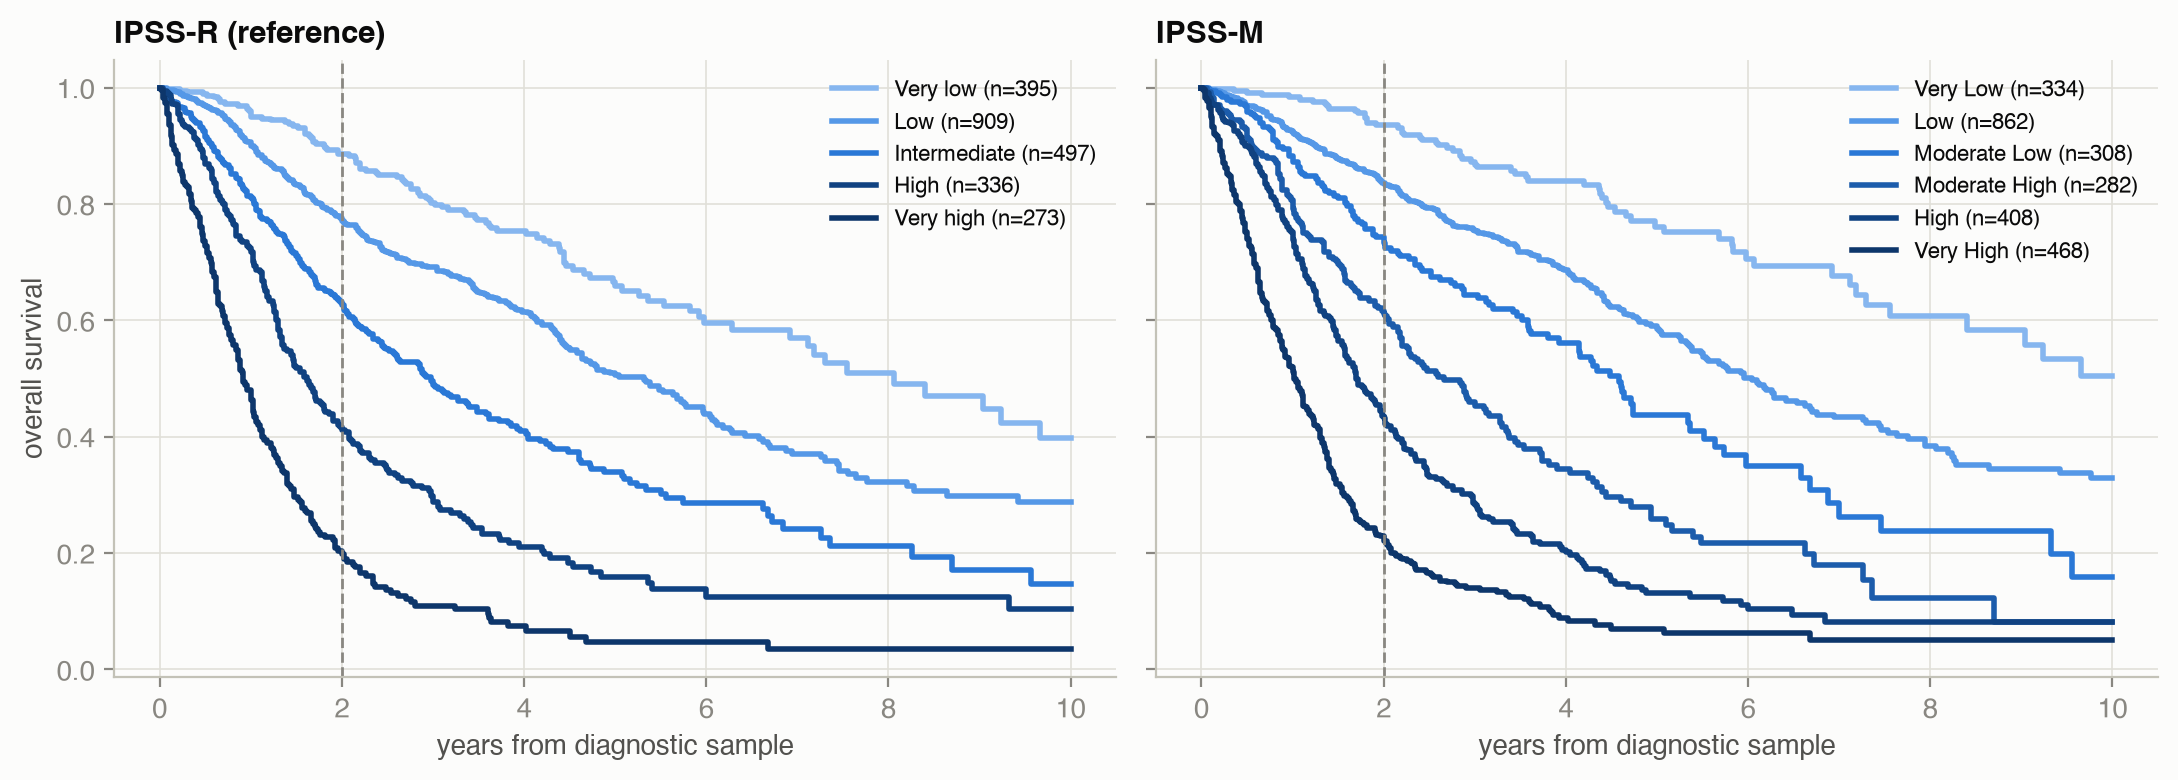
\includegraphics[width=\textwidth]{F1_km_reference_scores.png}
\caption{Overall survival by IPSS-R and IPSS-M group in the intended-use cohort (Kaplan--Meier); dashed line at 2 years.}
\end{figure}

\textbf{Questions for the referring haematologist.} Some facts cannot be inferred from the file; we would ask, in priority order: (1) were transplanted patients censored at transplant? (2) is time zero the diagnostic sample for every patient? (3) does an absent mutation row mean a negative panel or no panel? (4) which diagnoses are included (CMML, therapy-related MDS)? (5) were deaths ascertained the same way in every centre? (6) is 30\,\% the right referral threshold for the local transplant-related mortality? Pending answers we assumed, respectively: survival as recorded, time zero at diagnosis, wild type, MDS approximated by blasts and WBC, complete ascertainment, and the published IPSS-M boundary.

\section{Methods}
\textbf{Inputs and reference scores.} From the mutation panel we build one indicator per gene, TP53 multi-hit, the two SF3B1 subtypes and a count of residual driver genes, as defined by the official IPSS-M implementation~\cite{ipssmcode}. IPSS-R follows~\cite{ipssr,schanz}; our IPSS-M code reproduces the official package's test patients to the second decimal. Centre is never an input.

\textbf{Candidates}, simplest first: (1) IPSS-M recalibrated, with two numbers estimated locally (slope from score to hazard, 2-year baseline survival); (2) a Cox model refitted on the 22 IPSS-M variables (elastic net); (3) a Cox model on 35 variables, adding neutrophils, WBC, monocytes, karyotype and mutation counts and seven genes; (4) gradient-boosted survival trees on the same 35 inputs.

\textbf{Selection rule}, fixed before the comparison was first run: deploy the simplest candidate whose C-index is within 0.005 of the best, provided observed/expected 2-year deaths lies in 0.9--1.1.

\textbf{Validation.} Each model is fitted on 22 centres and scored on the 23rd; penalties are chosen by cross-validation across training centres only. On the pooled out-of-centre predictions we report Harrell's and Uno's C-index~\cite{uno}, the time-dependent AUC and Brier score at 2 years (inverse-probability-of-censoring weighted), observed/expected deaths, calibration slope and net benefit~\cite{vickers}, with 95\,\% bootstrap intervals (500 resamples; paired for differences). The 30\,\% threshold was fixed in advance as the 2-year risk at the IPSS-M Moderate-Low/Moderate-High boundary.

\section{Results}
\begin{table}[h]
\centering\small
\setlength{\tabcolsep}{4pt}
\caption{Performance on the head-to-head cohort (2{,}382 patients, 1{,}129 deaths), each centre held out.}\label{tab:metrics}
\begin{tabular}{@{}lcccccc@{}}
\toprule
Model & Harrell C (95\,\% CI) & Uno C & AUC 2 y (95\,\% CI) & Brier 2 y & O/E & Slope\\
\midrule
IPSS-R (reference) & 0.707 (0.691--0.723) & 0.688 & 0.754 (0.732--0.776) & 0.186 & 0.99 & 0.97\\
\textbf{IPSS-M, recalibrated} & \textbf{0.750 (0.735--0.766)} & \textbf{0.737} & \textbf{0.809 (0.790--0.830)} & \textbf{0.167} & \textbf{0.98} & \textbf{0.98}\\
Cox, 22 variables & 0.747 (0.733--0.762) & 0.734 & 0.806 (0.788--0.826) & 0.170 & 0.96 & 1.09\\
Cox, 35 variables & 0.746 (0.733--0.762) & 0.735 & 0.802 (0.782--0.823) & 0.171 & 0.96 & 1.16\\
Boosted trees & 0.742 (0.728--0.758) & 0.730 & 0.800 (0.779--0.821) & 0.171 & 0.95 & 1.13\\
\bottomrule
\end{tabular}
\end{table}

IPSS-M beats IPSS-R by $+0.043$ C-index (0.032--0.053). Against IPSS-M, the refitted models score $-0.003$ ($-0.007$ to $0.000$), $-0.004$ ($-0.008$ to $0.001$) and, for boosted trees, $-0.008$ ($-0.015$ to $-0.002$): extra variables bought nothing and flexibility cost a little. The rule therefore selects \textbf{IPSS-M, recalibrated}. Its home advantage is small: the refitted 22-variable model, which never sees the held-out centre, reaches 0.747, so we expect about 0.745 at a new centre.

\begin{figure}[h]
\centering
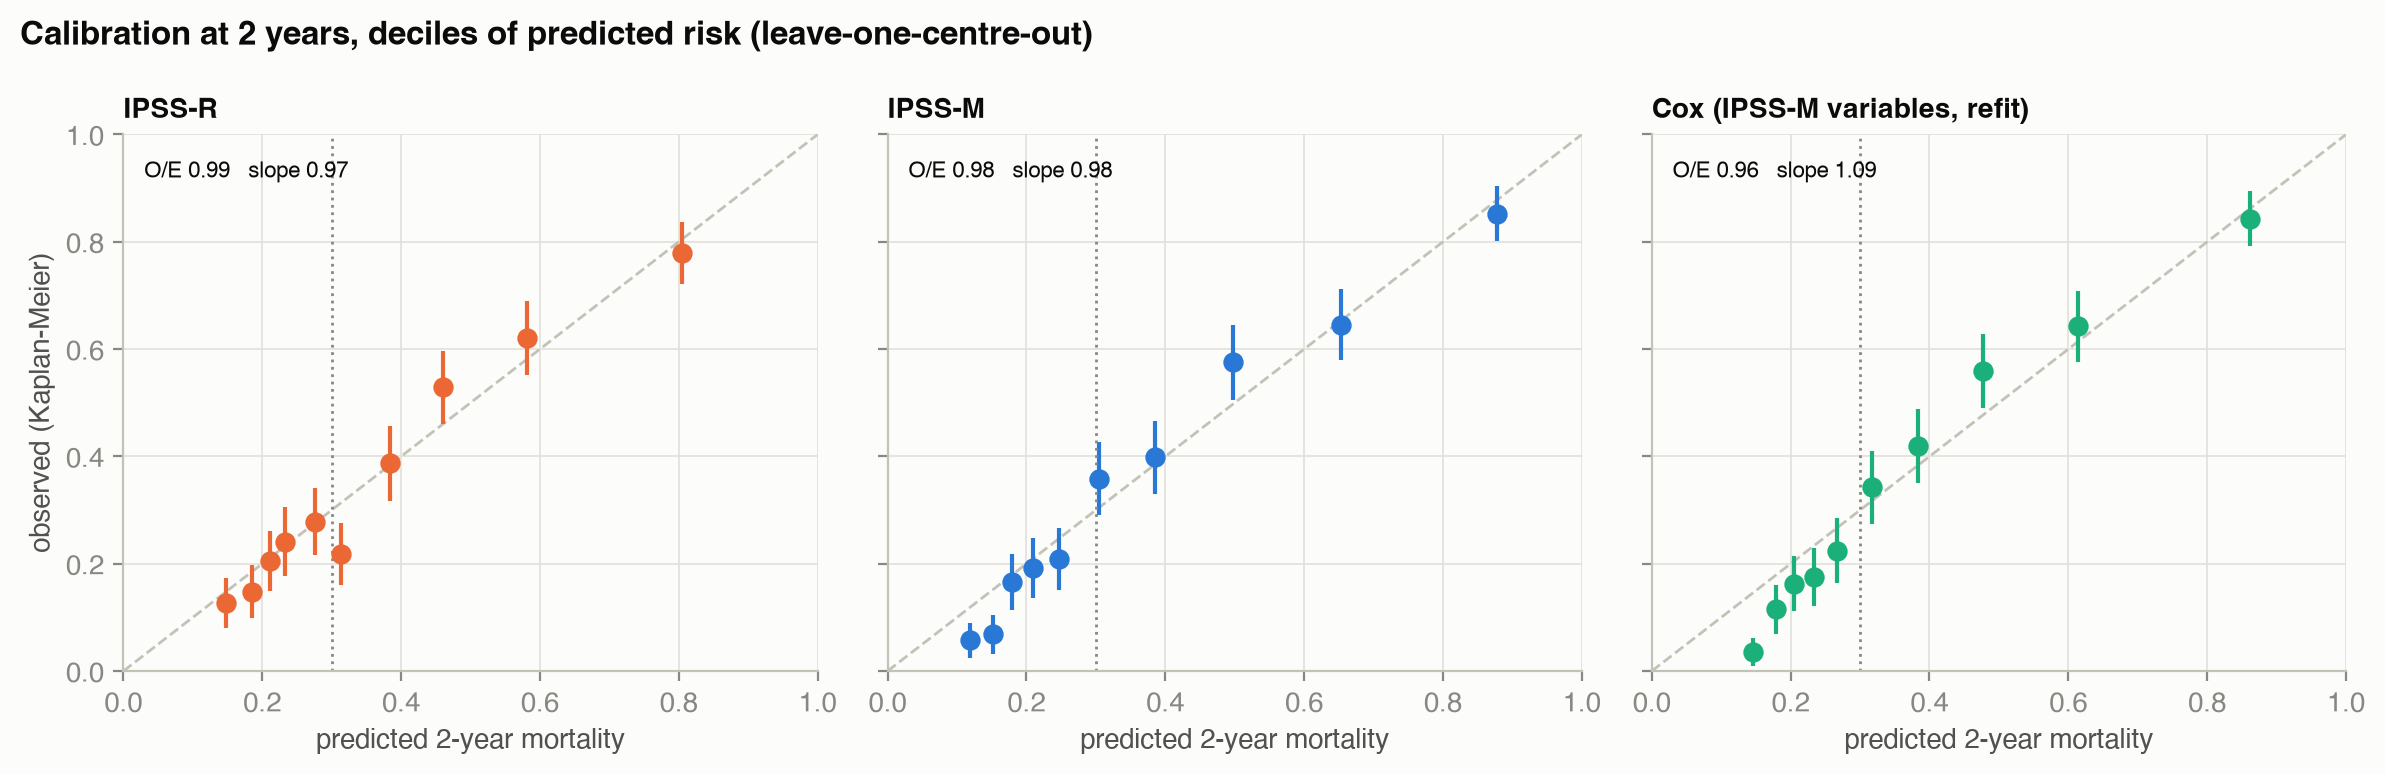
\includegraphics[width=\textwidth]{F6_calibration.png}
\caption{Calibration at 2 years by decile of predicted risk (Kaplan--Meier observed, 95\,\% intervals). The tool (middle) is calibrated overall; it overestimates risk only in the lowest-risk fifth (12--15\,\% predicted, 6--7\,\% observed), far below the threshold.}
\end{figure}

\begin{table}[h]
\centering\small
\setlength{\tabcolsep}{4.5pt}
\caption{Decision rules against death within 2 years (Kaplan--Meier estimates).}\label{tab:policy}
\begin{tabular}{@{}lccccc@{}}
\toprule
Rule & Flagged & Sensitivity & Specificity & Mortality if flagged & Survival if not\\
\midrule
IPSS-R $>3.5$ & 39.6\,\% & 65.1\,\% & 74.8\,\% & 58.5\,\% & 79.8\,\%\\
IPSS-M Moderate-High or worse & 43.5\,\% & 73.8\,\% & 74.0\,\% & 60.3\,\% & 84.4\,\%\\
\textbf{Tool: 2-year risk $\geq 30$\,\%} & \textbf{45.4\,\%} & \textbf{75.5\,\%} & \textbf{71.8\,\%} & \textbf{59.2\,\%} & \textbf{84.8\,\%}\\
\bottomrule
\end{tabular}
\end{table}

At 30\,\% the tool's net benefit is 0.189, against 0.159 for IPSS-R and 0.079 for referring everyone: three more patients who die within 2 years correctly brought to the transplant discussion per 100, with no net increase in false flags. The advantage holds at every threshold from 8\,\% to 65\,\% (Figure~\ref{fig:dca}). Compared with the IPSS-R rule, 253 patients move up (2-year mortality 45.7\,\%; they carry ASXL1, RUNX1, SRSF2 and EZH2 mutations far more often) and 115 move down (21.2\,\%).

\begin{figure}[h]
\centering
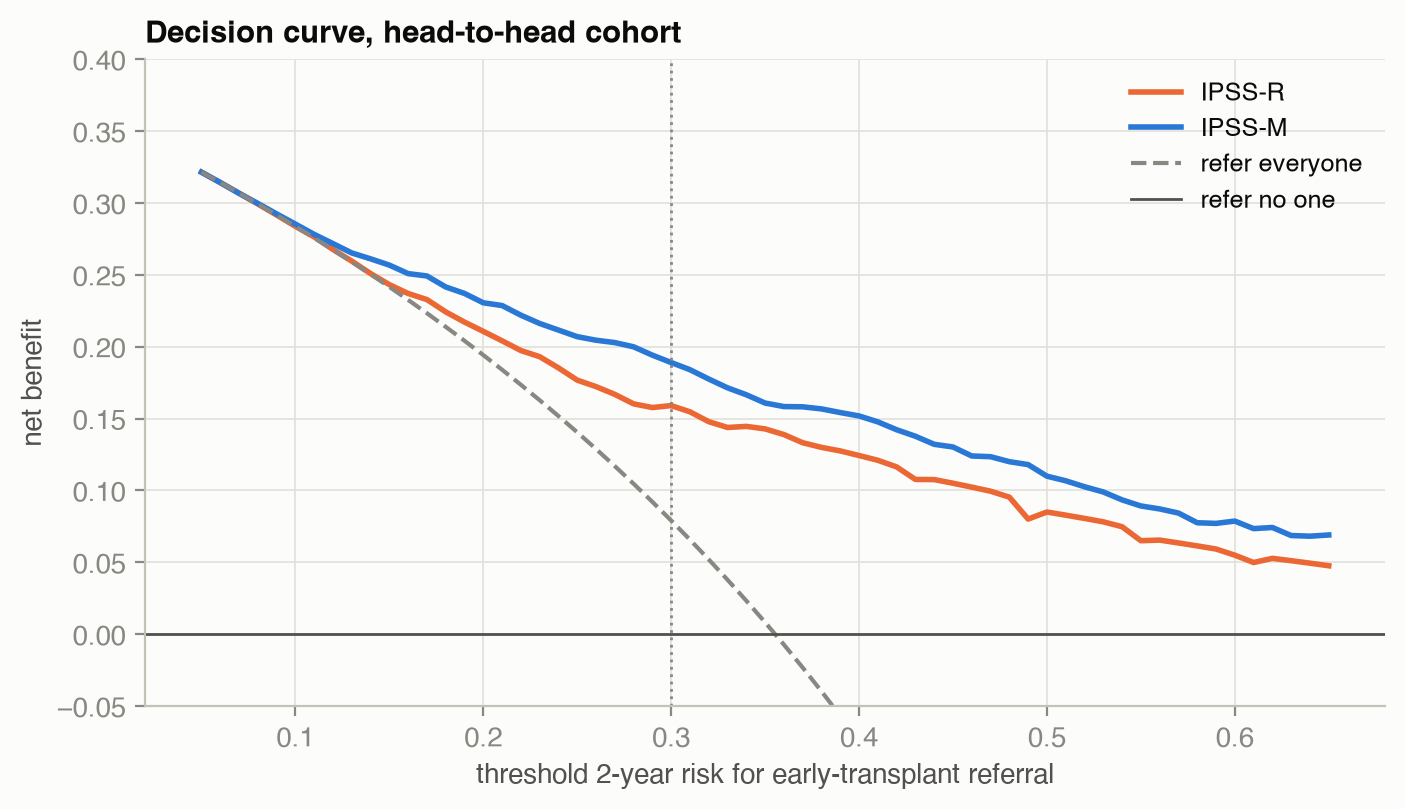
\includegraphics[width=0.72\textwidth]{F7_decision_curve.png}
\caption{Decision curve: net benefit of referring for early transplant when the predicted 2-year risk exceeds each threshold.}\label{fig:dca}
\end{figure}

\section{The model and the tool}
The whole model is
\[
\text{2-year risk of death} \approx 1 - 0.684^{\,\exp(0.57 \times \text{IPSS-M score})},
\]
where the IPSS-M score is the published weighted sum of 22 inputs; only the slope (0.57 per point) and the baseline were fitted here. The 30\,\% threshold falls at score $-0.07$, almost exactly the Moderate-Low/Moderate-High boundary (31.6\,\% at score 0). Table~\ref{tab:weights} gives the effects; recalibration shrinks each one by the same power (0.83) and keeps their order. Neutrophils, WBC, monocytes and genes such as TET2 are not used.

\begin{table}[h]
\centering\small
\setlength{\tabcolsep}{4pt}
\caption{Hazard ratio per unit: published IPSS-M / after recalibration in this cohort.}\label{tab:weights}
\begin{tabular}{@{}lcc@{\hspace{0.8cm}}lcc@{}}
\toprule
Feature & Published & Cohort & Feature & Published & Cohort\\
\midrule
Haemoglobin (per g/dL) & 0.84 & 0.87 & NRAS & 1.52 & 1.41\\
Platelets (per $100\times10^9$/L) & 0.80 & 0.83 & ETV6 & 1.48 & 1.38\\
Marrow blasts (per 5\,\%) & 1.42 & 1.34 & IDH2 & 1.46 & 1.37\\
Karyotype group (per IPSS-R step) & 1.33 & 1.27 & CBL & 1.34 & 1.28\\
\textbf{TP53 multi-hit} & \textbf{3.25} & \textbf{2.65} & EZH2 & 1.31 & 1.25\\
FLT3 & 2.22 & 1.94 & U2AF1 & 1.28 & 1.23\\
KMT2A partial tandem duplication & 2.22 & 1.94 & SRSF2 & 1.27 & 1.22\\
SF3B1 with isolated del(5q) & 1.66 & 1.52 & DNMT3A & 1.25 & 1.20\\
NPM1 & 1.54 & 1.43 & ASXL1 & 1.24 & 1.19\\
RUNX1 & 1.53 & 1.42 & KRAS & 1.22 & 1.18\\
Other driver genes (per gene, max 2) & 1.26 & 1.21 & SF3B1, favourable form & 0.92 & 0.94\\
\bottomrule
\end{tabular}
\end{table}

Each patient gets a risk, a range combining bootstrap uncertainty of the two local numbers with the best and worst values of any missing input, and a band set by where the whole range falls. In the intended-use cohort 47.7\,\% are Lower risk (observed 2-year mortality 14.3\,\%), 42.4\,\% Higher (61.1\,\%) and 9.8\,\% Borderline (28.7\,\%), mostly because the karyotype is missing (63\,\% of borderline patients). Figure~\ref{fig:card} shows a card: IPSS-R calls this patient Intermediate, while a del(3q) karyotype with RUNX1, EZH2 and ASXL1 mutations gives 63\,\%, and IPSS-M agrees (Very High).

\begin{figure}[h]
\centering
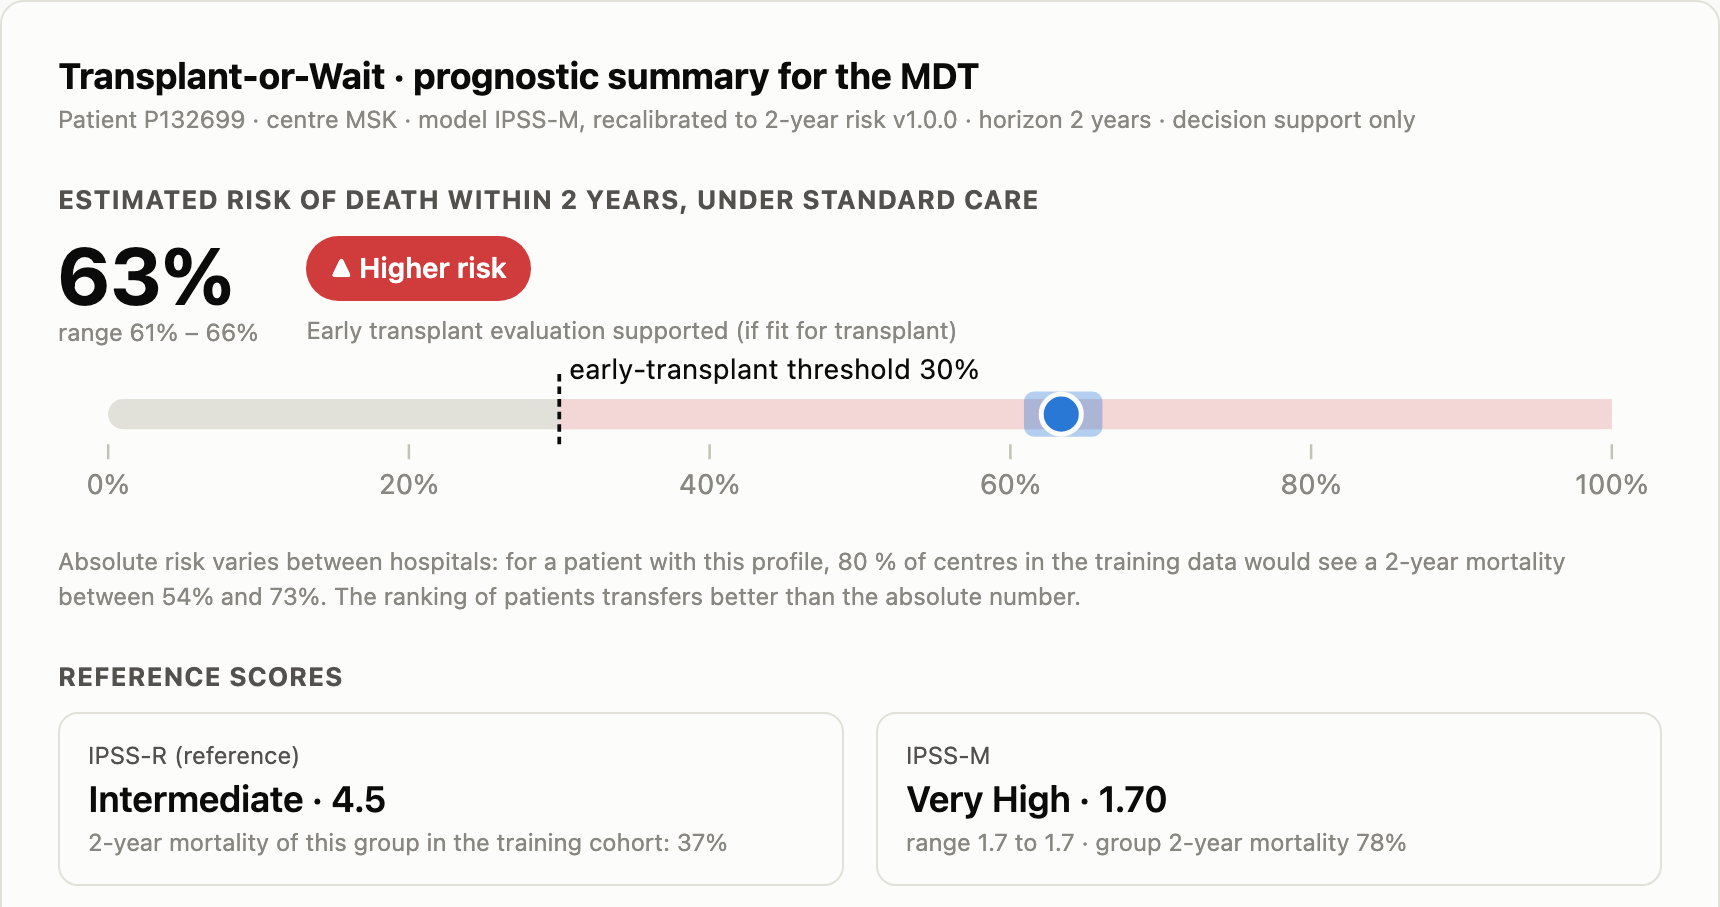
\includegraphics[width=0.8\textwidth]{F10_card_P132699_top.png}
\caption{Top of the patient card for one higher-risk patient. The full card adds the drivers of the estimate, the inputs used, warnings and the tool's limits.}\label{fig:card}
\end{figure}

\section{Where performance degrades}\label{sec:fail}
\begin{table}[h]
\centering\small
\caption{Failure modes (out-of-centre predictions, IPSS-M recalibrated).}
\begin{tabularx}{\textwidth}{@{}lrccL@{}}
\toprule
Condition & Patients & C-index & O/E & Response of the tool\\
\midrule
A given centre (18 with $\geq15$ deaths) & -- & 0.67--0.86 & 0.57--1.41 & Shows the range 80\,\% of centres would see; recalibrate locally\\
Lower-risk group (score $\leq 0$) & 1{,}504 & 0.63 & 0.83 & Band only, no finer ranking\\
Karyotype missing & 252 & 0.73 & 1.16 & Widens the range, usually Borderline\\
No mutation recorded & 244 & 0.67 & 0.91 & Asks to confirm the panel was run\\
Monocytosis (possible CMML) & 337 & 0.73 & 0.89 & Warns to check CMML criteria\\
Short-follow-up centres & 703 & 0.81 & 0.69 & Possible missed deaths: a monitoring item\\
Out of scope: blasts $\geq 20$\,\% & 152 & 0.66 & 0.84 & Band ``Out of intended use''\\
Out of scope: WBC $\geq 13\times10^9$/L & 198 & 0.68 & 1.12 & Band ``Out of intended use''\\
\bottomrule
\end{tabularx}
\end{table}

The ranking holds across subgroups and centres; the absolute number does not (between-centre spread $\tau=0.21$ on the log-hazard scale), and two failure modes cannot be measured here: a later period (the file has no dates) and a centre unlike all 23.

\section{Deployment and responsibility}
The tool gives a prognosis for an individual patient to inform a therapeutic decision, so it is medical device software (MDR Art.~2(1)); since a wrong output can cost a life, we argue class III under Rule~11. Used only inside the hospital it could follow the in-house route (MDR Art.~5(5)); it is a high-risk system under the AI Act, whose obligations for medical devices apply from 2 August 2028. Health data are a special category (GDPR Art.~9): a data protection impact assessment is needed and the tool runs on hospital servers or an HDS-certified host. Against automation bias, the card shows IPSS-R and IPSS-M beside the estimate, gives no advice when borderline and states what the tool cannot know (fitness, age, donor). Monitoring: input means and missing karyotypes monthly; the share at $\geq 30$\,\% quarterly (alarm outside 35--55\,\%); observed/expected deaths every 6 months (alarm outside 0.8--1.25); every Lower-risk patient who dies within 2 years reviewed. Go-live only after a 3-month silent run, local recalibration (pre-specified as a planned change), and with a named haematologist who owns the tool and can switch it off.

\section{Pre-registration for the held-out test set}
Written before the test set is scored, for intended-use patients drawn from the same centres: Harrell C-index 0.745 (we accept 0.72--0.77); AUC at 2 years 0.80 (0.77--0.83); observed/expected 2-year deaths 0.85--1.15 (0.55--1.45 if one or two centres only); bands about 48\,\% Lower, 42\,\% Higher, 10\,\% Borderline. \textbf{The error we cannot accept} is a Lower-risk call for a patient who dies within 2 years: we pre-register a Lower-band 2-year mortality of at most 18\,\% (training 14.3\,\%) and no TP53 multi-hit patient in the Lower band (0 of 179 in training). The test set is scored with \texttt{scripts/predict.py}; its \texttt{risk\_score} column ranks patients for the C-index.

\section{Limitations}
There is no external validation: the file overlaps the IPSS-M development cohort and holding out a centre is the furthest we could go. Treatment is invisible: if transplanted patients were followed after transplant, the risk without transplant is understated in the higher-risk groups. The outcome is all-cause death only, and sequencing panels and karyotype formats vary by laboratory. To answer ``transplant or wait'' itself, the department would need treatment and transplant dates, age, performance status, comorbidity (HCT-CI), donor availability and progression to AML; immediate and delayed transplant could then be compared with a multistate model or a target-trial emulation, as in~\cite{tentori}.

\textbf{Reproducibility.} \path{run_all.sh} rebuilds every number and figure from the two data files in about 4 minutes. The data audit and the model comparison run in the notebooks \path{01_data_audit} and \path{02_model_comparison}; the script \path{03_train_final.py} freezes the model; the notebook \path{03_final_model_and_tool} explains it. Random seeds are fixed; tests check the karyotype parser and the IPSS-M implementation.

{\small
\begin{thebibliography}{9}\setlength{\itemsep}{0pt}
\bibitem{ipssr} Greenberg PL, et al. Revised International Prognostic Scoring System for myelodysplastic syndromes. \emph{Blood} 2012;120:2454--65.
\bibitem{ipssm} Bernard E, et al. Molecular International Prognostic Scoring System for myelodysplastic syndromes. \emph{NEJM Evidence} 2022;1(7).
\bibitem{tentori} Tentori CA, et al. Clinical and genomic-based decision support system to define the optimal timing of allogeneic hematopoietic stem-cell transplantation in patients with myelodysplastic syndromes. \emph{J Clin Oncol} 2024;42:2873--86.
\bibitem{schanz} Schanz J, et al. New comprehensive cytogenetic scoring system for primary myelodysplastic syndromes. \emph{J Clin Oncol} 2012;30:820--9.
\bibitem{wiens} Wiens J, et al. Do no harm: a roadmap for responsible machine learning for health care. \emph{Nat Med} 2019;25:1337--40.
\bibitem{uno} Uno H, et al. On the C-statistics for evaluating overall adequacy of risk prediction procedures with censored survival data. \emph{Stat Med} 2011;30:1105--17.
\bibitem{vickers} Vickers AJ, Elkin EB. Decision curve analysis. \emph{Med Decis Making} 2006;26:565--74.
\bibitem{ipssmcode} Official IPSS-M implementation, \url{https://github.com/papaemmelab/ipssm}.
\bibitem{acs} American Cancer Society. Survival statistics for myelodysplastic syndromes (IPSS-M group medians).
\end{thebibliography}}

\end{document}
